\documentclass[]{ctexbook}
\usepackage{lmodern}
\usepackage{amssymb,amsmath}
\usepackage{ifxetex,ifluatex}
\usepackage{fixltx2e} % provides \textsubscript
\ifnum 0\ifxetex 1\fi\ifluatex 1\fi=0 % if pdftex
  \usepackage[T1]{fontenc}
  \usepackage[utf8]{inputenc}
\else % if luatex or xelatex
  \ifxetex
    \usepackage{xltxtra,xunicode}
  \else
    \usepackage{fontspec}
  \fi
  \defaultfontfeatures{Ligatures=TeX,Scale=MatchLowercase}
\fi
% use upquote if available, for straight quotes in verbatim environments
\IfFileExists{upquote.sty}{\usepackage{upquote}}{}
% use microtype if available
\IfFileExists{microtype.sty}{%
\usepackage{microtype}
\UseMicrotypeSet[protrusion]{basicmath} % disable protrusion for tt fonts
}{}
\usepackage[b5paper,tmargin=2.5cm,bmargin=2.5cm,lmargin=3.5cm,rmargin=2.5cm]{geometry}
\usepackage[unicode=true]{hyperref}
\PassOptionsToPackage{usenames,dvipsnames}{color} % color is loaded by hyperref
\hypersetup{
            pdftitle={Overleaf功能介绍},
            pdfauthor={wang},
            colorlinks=true,
            linkcolor=Maroon,
            citecolor=Blue,
            urlcolor=Blue,
            breaklinks=true}
\urlstyle{same}  % don't use monospace font for urls
\usepackage{natbib}
\bibliographystyle{apalike}
\usepackage{color}
\usepackage{fancyvrb}
\newcommand{\VerbBar}{|}
\newcommand{\VERB}{\Verb[commandchars=\\\{\}]}
\DefineVerbatimEnvironment{Highlighting}{Verbatim}{commandchars=\\\{\}}
% Add ',fontsize=\small' for more characters per line
\usepackage{framed}
\definecolor{shadecolor}{RGB}{248,248,248}
\newenvironment{Shaded}{\begin{snugshade}}{\end{snugshade}}
\newcommand{\AlertTok}[1]{\textcolor[rgb]{0.94,0.16,0.16}{#1}}
\newcommand{\AnnotationTok}[1]{\textcolor[rgb]{0.56,0.35,0.01}{\textbf{\textit{#1}}}}
\newcommand{\AttributeTok}[1]{\textcolor[rgb]{0.77,0.63,0.00}{#1}}
\newcommand{\BaseNTok}[1]{\textcolor[rgb]{0.00,0.00,0.81}{#1}}
\newcommand{\BuiltInTok}[1]{#1}
\newcommand{\CharTok}[1]{\textcolor[rgb]{0.31,0.60,0.02}{#1}}
\newcommand{\CommentTok}[1]{\textcolor[rgb]{0.56,0.35,0.01}{\textit{#1}}}
\newcommand{\CommentVarTok}[1]{\textcolor[rgb]{0.56,0.35,0.01}{\textbf{\textit{#1}}}}
\newcommand{\ConstantTok}[1]{\textcolor[rgb]{0.00,0.00,0.00}{#1}}
\newcommand{\ControlFlowTok}[1]{\textcolor[rgb]{0.13,0.29,0.53}{\textbf{#1}}}
\newcommand{\DataTypeTok}[1]{\textcolor[rgb]{0.13,0.29,0.53}{#1}}
\newcommand{\DecValTok}[1]{\textcolor[rgb]{0.00,0.00,0.81}{#1}}
\newcommand{\DocumentationTok}[1]{\textcolor[rgb]{0.56,0.35,0.01}{\textbf{\textit{#1}}}}
\newcommand{\ErrorTok}[1]{\textcolor[rgb]{0.64,0.00,0.00}{\textbf{#1}}}
\newcommand{\ExtensionTok}[1]{#1}
\newcommand{\FloatTok}[1]{\textcolor[rgb]{0.00,0.00,0.81}{#1}}
\newcommand{\FunctionTok}[1]{\textcolor[rgb]{0.00,0.00,0.00}{#1}}
\newcommand{\ImportTok}[1]{#1}
\newcommand{\InformationTok}[1]{\textcolor[rgb]{0.56,0.35,0.01}{\textbf{\textit{#1}}}}
\newcommand{\KeywordTok}[1]{\textcolor[rgb]{0.13,0.29,0.53}{\textbf{#1}}}
\newcommand{\NormalTok}[1]{#1}
\newcommand{\OperatorTok}[1]{\textcolor[rgb]{0.81,0.36,0.00}{\textbf{#1}}}
\newcommand{\OtherTok}[1]{\textcolor[rgb]{0.56,0.35,0.01}{#1}}
\newcommand{\PreprocessorTok}[1]{\textcolor[rgb]{0.56,0.35,0.01}{\textit{#1}}}
\newcommand{\RegionMarkerTok}[1]{#1}
\newcommand{\SpecialCharTok}[1]{\textcolor[rgb]{0.00,0.00,0.00}{#1}}
\newcommand{\SpecialStringTok}[1]{\textcolor[rgb]{0.31,0.60,0.02}{#1}}
\newcommand{\StringTok}[1]{\textcolor[rgb]{0.31,0.60,0.02}{#1}}
\newcommand{\VariableTok}[1]{\textcolor[rgb]{0.00,0.00,0.00}{#1}}
\newcommand{\VerbatimStringTok}[1]{\textcolor[rgb]{0.31,0.60,0.02}{#1}}
\newcommand{\WarningTok}[1]{\textcolor[rgb]{0.56,0.35,0.01}{\textbf{\textit{#1}}}}
\usepackage{longtable,booktabs}
% Fix footnotes in tables (requires footnote package)
\IfFileExists{footnote.sty}{\usepackage{footnote}\makesavenoteenv{long table}}{}
\IfFileExists{parskip.sty}{%
\usepackage{parskip}
}{% else
\setlength{\parindent}{0pt}
\setlength{\parskip}{6pt plus 2pt minus 1pt}
}
\setlength{\emergencystretch}{3em}  % prevent overfull lines
\providecommand{\tightlist}{%
  \setlength{\itemsep}{0pt}\setlength{\parskip}{0pt}}
\setcounter{secnumdepth}{5}
% Redefines (sub)paragraphs to behave more like sections
\ifx\paragraph\undefined\else
\let\oldparagraph\paragraph
\renewcommand{\paragraph}[1]{\oldparagraph{#1}\mbox{}}
\fi
\ifx\subparagraph\undefined\else
\let\oldsubparagraph\subparagraph
\renewcommand{\subparagraph}[1]{\oldsubparagraph{#1}\mbox{}}
\fi

% set default figure placement to htbp
\makeatletter
\def\fps@figure{htbp}
\makeatother

\usepackage{booktabs}
\usepackage{longtable}

\usepackage{framed,color}
\definecolor{shadecolor}{RGB}{248,248,248}

\renewcommand{\textfraction}{0.05}
\renewcommand{\topfraction}{0.8}
\renewcommand{\bottomfraction}{0.8}
\renewcommand{\floatpagefraction}{0.75}

\let\oldhref\href
\renewcommand{\href}[2]{#2\footnote{\url{#1}}}

\makeatletter
\newenvironment{kframe}{%
\medskip{}
\setlength{\fboxsep}{.8em}
 \def\at@end@of@kframe{}%
 \ifinner\ifhmode%
  \def\at@end@of@kframe{\end{minipage}}%
  \begin{minipage}{\columnwidth}%
 \fi\fi%
 \def\FrameCommand##1{\hskip\@totalleftmargin \hskip-\fboxsep
 \colorbox{shadecolor}{##1}\hskip-\fboxsep
     % There is no \\@totalrightmargin, so:
     \hskip-\linewidth \hskip-\@totalleftmargin \hskip\columnwidth}%
 \MakeFramed {\advance\hsize-\width
   \@totalleftmargin\z@ \linewidth\hsize
   \@setminipage}}%
 {\par\unskip\endMakeFramed%
 \at@end@of@kframe}
\makeatother

\makeatletter
\@ifundefined{Shaded}{
}{\renewenvironment{Shaded}{\begin{kframe}}{\end{kframe}}}
\@ifpackageloaded{fancyvrb}{%
  % https://github.com/CTeX-org/ctex-kit/issues/331
  \RecustomVerbatimEnvironment{Highlighting}{Verbatim}{commandchars=\\\{\},formatcom=\xeCJKVerbAddon}%
}{}
\makeatother

\usepackage{makeidx}
\makeindex

\urlstyle{tt}

\usepackage{amsthm}
\makeatletter
\def\thm@space@setup{%
  \thm@preskip=8pt plus 2pt minus 4pt
  \thm@postskip=\thm@preskip
}
\makeatother

\frontmatter

\title{Overleaf功能介绍}
\author{wang}
\date{2019-06-01}

\let\BeginKnitrBlock\begin \let\EndKnitrBlock\end
\begin{document}
\maketitle


\thispagestyle{empty}

\begin{center}
献给……

呃,爱谁谁吧
\end{center}

\setlength{\abovedisplayskip}{-5pt}
\setlength{\abovedisplayshortskip}{-5pt}

{
\setcounter{tocdepth}{2}
\tableofcontents
}
\listoftables
\listoffigures
\hypertarget{section}{%
\chapter*{前言}\label{section}}


Overleaf是什么

\url{https://www.overleaf.com/}

简单讲,Overleaf是一个在线的LaTeX环境.
不需要在自己电脑上安装,通过网页访问即可编写LaTeX.

如果还不了解LaTeX,可以先阅读下面的链接:

LaTeX的介绍:
\url{https://liam.page/2014/09/08/latex-introduction/}

当然,Overleaf提供的服务远不止此.

借助Overleaf,可以实现多人合作编辑,无缝同步进度,追踪文件修改历史.

你好,世界。我写了一本书。这本书是这样的,第 \ref{intro} 章介绍了啥啥,第 \ref{wind} 章说了啥啥,然后是啥啥\ldots{}\ldots{}

我用了两个 R 包编译这本书,分别是 \textbf{knitr}\index{knitr} \citep{xie2015} 和 \textbf{bookdown}\index{bookdown} \citep{R-bookdown}。以下是我的 R 进程信息:

\begin{Shaded}
\begin{Highlighting}[]
\KeywordTok{sessionInfo}\NormalTok{()}
\end{Highlighting}
\end{Shaded}

\begin{verbatim}
## R version 3.6.0 (2019-04-26)
## Platform: x86_64-apple-darwin15.6.0 (64-bit)
## Running under: macOS Mojave 10.14.5
## 
## Matrix products: default
## BLAS:   /Library/Frameworks/R.framework/Versions/3.6/Resources/lib/libRblas.0.dylib
## LAPACK: /Library/Frameworks/R.framework/Versions/3.6/Resources/lib/libRlapack.dylib
## 
## locale:
## [1] en_US.UTF-8/en_US.UTF-8/en_US.UTF-8/C/en_US.UTF-8/en_US.UTF-8
## 
## attached base packages:
## [1] stats     graphics  grDevices utils     datasets 
## [6] methods   base     
## 
## other attached packages:
## [1] xtable_1.8-4
## 
## loaded via a namespace (and not attached):
##  [1] compiler_3.6.0  magrittr_1.5    bookdown_0.11  
##  [4] tools_3.6.0     htmltools_0.3.6 rstudioapi_0.10
##  [7] yaml_2.2.0      Rcpp_1.0.1      stringi_1.4.3  
## [10] rmarkdown_1.13  highr_0.8       knitr_1.23     
## [13] stringr_1.4.0   xfun_0.7        digest_0.6.18  
## [16] evaluate_0.14
\end{verbatim}

\hypertarget{section-1}{%
\section*{致谢}\label{section-1}}


非常感谢谁谁以及谁谁对我的帮助。艾玛,要不是他们神一样的队友,我两年前就写完这本书了。

\BeginKnitrBlock{flushright}
张三\\
于 A 村某角落
\EndKnitrBlock{flushright}

\hypertarget{author}{%
\chapter*{作者简介}\label{author}}


上不了厅堂,下得了厨房。敲得了代码,逮得住蟑螂。

\mainmatter

\hypertarget{intro}{%
\chapter{Overleaf写作流程}\label{intro}}

\hypertarget{section-2}{%
\section{创建项目}\label{section-2}}

空白文档
GitHub
\ldots{}

\hypertarget{section-3}{%
\section{个人写作}\label{section-3}}

\hypertarget{section-4}{%
\section{邀请合作者}\label{section-4}}

\hypertarget{section-5}{%
\section{论文投递}\label{section-5}}

现在我们可以试试 \textbf{bookdown} 的一些初级功能了,例如图表。图 \ref{fig:hello} 是一幅无趣的散点图,表 \ref{tab:iris} 是一份枯燥的数据。

\begin{Shaded}
\begin{Highlighting}[]
\KeywordTok{par}\NormalTok{(}\DataTypeTok{mar =} \KeywordTok{c}\NormalTok{(}\DecValTok{4}\NormalTok{, }\DecValTok{4}\NormalTok{, }\DecValTok{1}\NormalTok{, }\FloatTok{.1}\NormalTok{))}
\KeywordTok{plot}\NormalTok{(cars, }\DataTypeTok{pch =} \DecValTok{19}\NormalTok{)}
\end{Highlighting}
\end{Shaded}

\begin{figure}
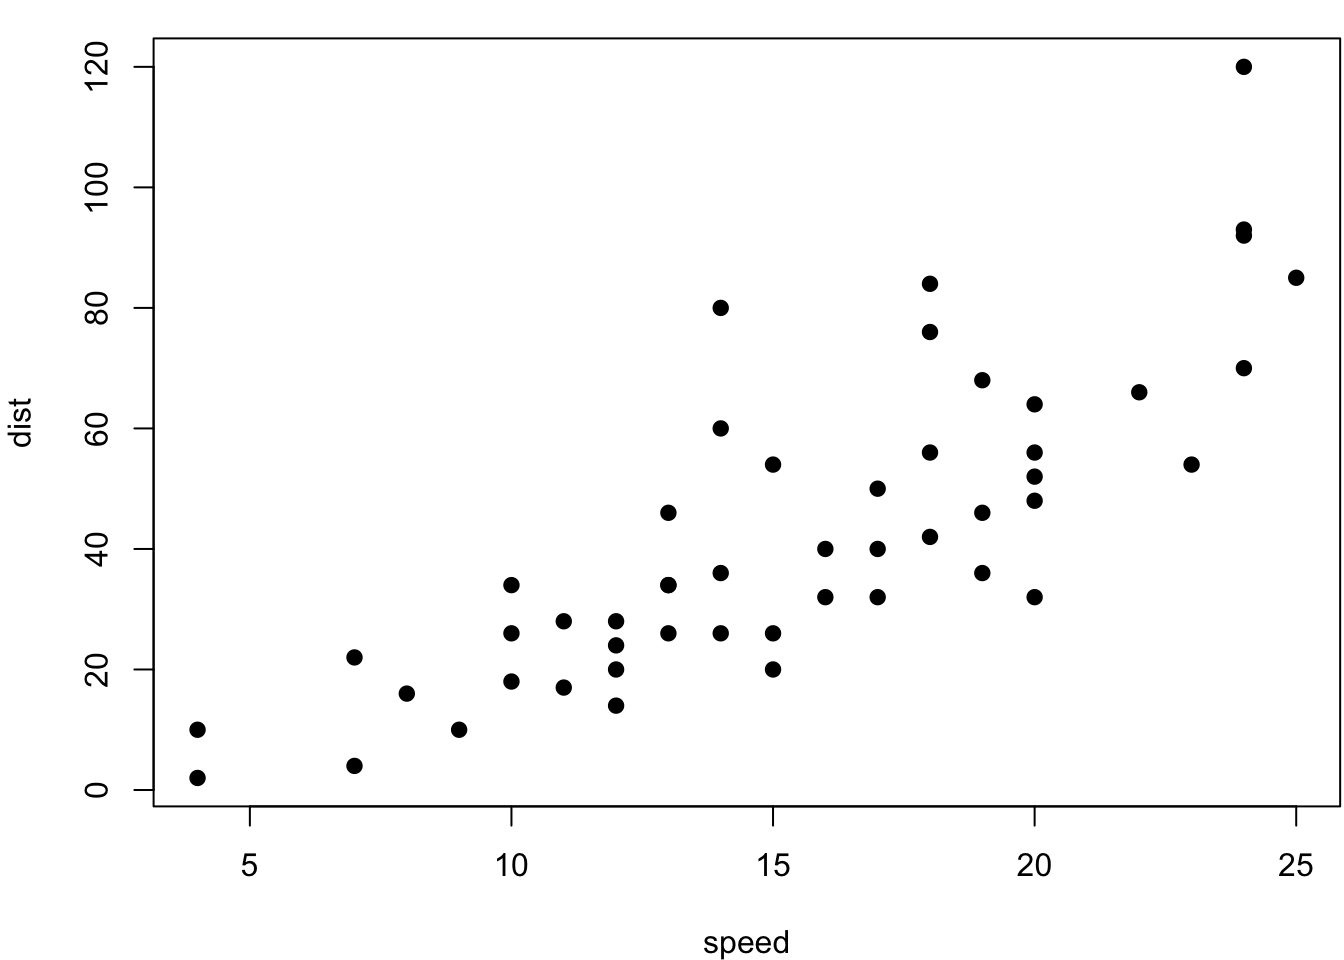
\includegraphics[width=0.9\linewidth]{bookdown_files/figure-latex/hello-1} \caption{雷猴啊,散点图!}\label{fig:hello}
\end{figure}

\begin{Shaded}
\begin{Highlighting}[]
\NormalTok{knitr}\OperatorTok{::}\KeywordTok{kable}\NormalTok{(}
  \KeywordTok{head}\NormalTok{(iris), }\DataTypeTok{caption =} \StringTok{'雷猴啊,iris 数据!'}\NormalTok{,}
  \DataTypeTok{booktabs =} \OtherTok{TRUE}
\NormalTok{)}
\end{Highlighting}
\end{Shaded}

\begin{table}[t]

\caption{\label{tab:iris}雷猴啊,iris 数据!}
\centering
\begin{tabular}{rrrrl}
\toprule
Sepal.Length & Sepal.Width & Petal.Length & Petal.Width & Species\\
\midrule
5.1 & 3.5 & 1.4 & 0.2 & setosa\\
4.9 & 3.0 & 1.4 & 0.2 & setosa\\
4.7 & 3.2 & 1.3 & 0.2 & setosa\\
4.6 & 3.1 & 1.5 & 0.2 & setosa\\
5.0 & 3.6 & 1.4 & 0.2 & setosa\\
\addlinespace
5.4 & 3.9 & 1.7 & 0.4 & setosa\\
\bottomrule
\end{tabular}
\end{table}

就这样,你可以一直编下去,直到编不下去。

\hypertarget{section-6}{%
\chapter{特色功能展示}\label{section-6}}

\hypertarget{section-7}{%
\section{本地和服务器同步}\label{section-7}}

\hypertarget{section-8}{%
\section{合作编辑}\label{section-8}}

\hypertarget{section-9}{%
\section{历史版本}\label{section-9}}

\hypertarget{section-10}{%
\section{参考文献整合}\label{section-10}}

张老爷子

话说张老爷子写了一首诗:

\begin{quote}
姑苏开遍碧桃时,邂逅河阳女画师。\\
红豆江南留梦影,白苹风末唱秋词。
\end{quote}

彭大将领

貌似大家都喜欢用白萍风这个意境。又如彭玉麟的对联:

\begin{quote}
凭栏看云影波光,最好是红蓼花疏、白苹秋老;\\
把酒对琼楼玉宇,莫孤负天心月到、水面风来。
\end{quote}

嘿,玛尼玛尼哄。

\hypertarget{section-11}{%
\chapter{订阅费用}\label{section-11}}

\url{https://www.overleaf.com/user/subscription/plans}

张老爷子

话说张老爷子写了一首诗:

\begin{quote}
姑苏开遍碧桃时,邂逅河阳女画师。\\
红豆江南留梦影,白苹风末唱秋词。
\end{quote}

彭大将领

貌似大家都喜欢用白萍风这个意境。又如彭玉麟的对联:

\begin{quote}
凭栏看云影波光,最好是红蓼花疏、白苹秋老;\\
把酒对琼楼玉宇,莫孤负天心月到、水面风来。
\end{quote}

嘿,玛尼玛尼哄。

\hypertarget{section-12}{%
\chapter{特色功能展示}\label{section-12}}

\hypertarget{section-13}{%
\section{本地和服务器同步}\label{section-13}}

\hypertarget{section-14}{%
\section{合作编辑}\label{section-14}}

\hypertarget{section-15}{%
\section{历史版本}\label{section-15}}

\hypertarget{section-16}{%
\section{参考文献整合}\label{section-16}}

张老爷子

话说张老爷子写了一首诗:

\begin{quote}
姑苏开遍碧桃时,邂逅河阳女画师。\\
红豆江南留梦影,白苹风末唱秋词。
\end{quote}

彭大将领

貌似大家都喜欢用白萍风这个意境。又如彭玉麟的对联:

\begin{quote}
凭栏看云影波光,最好是红蓼花疏、白苹秋老;\\
把酒对琼楼玉宇,莫孤负天心月到、水面风来。
\end{quote}

嘿,玛尼玛尼哄。

\hypertarget{section-17}{%
\chapter{其他工具}\label{section-17}}

这里介绍一些可以提高LaTeX写作效率的其他工具

\hypertarget{section-18}{%
\section{公式}\label{section-18}}

mathpix

可以很方便的将图片公式转成LaTex形式,手写笔记不太乱的话也是可以识别的.

\url{https://mathpix.com}

\hypertarget{section-19}{%
\section{表格}\label{section-19}}

在LaTeX中插入表格并不是很简单的一件事,尤其是当表头需要合并单元格时.
这里介绍一些可以提高输入表格效率的工具.

\hypertarget{xtable}{%
\subsection{xtable包}\label{xtable}}

在R中进行模拟时,将结果输出至LaTeX可以利用这个包中的xtable函数.

\url{https://cran.r-project.org/web/packages/xtable/index.html}

\begin{Shaded}
\begin{Highlighting}[]
\NormalTok{xtable}\OperatorTok{::}\KeywordTok{xtable}\NormalTok{(}\KeywordTok{matrix}\NormalTok{(}\KeywordTok{rnorm}\NormalTok{(}\DecValTok{12}\NormalTok{),}\DecValTok{3}\NormalTok{,}\DecValTok{4}\NormalTok{))}
\end{Highlighting}
\end{Shaded}

\begin{verbatim}
## % latex table generated in R 3.6.0 by xtable 1.8-4 package
## % Sat Jun  1 19:08:00 2019
## \begin{table}[ht]
## \centering
## \begin{tabular}{rrrrr}
##   \hline
##  & 1 & 2 & 3 & 4 \\ 
##   \hline
## 1 & -0.11 & 0.75 & -0.98 & -1.81 \\ 
##   2 & -1.08 & -0.60 & -0.57 & -1.55 \\ 
##   3 & -1.11 & 1.49 & 0.30 & 1.10 \\ 
##    \hline
## \end{tabular}
## \end{table}
\end{verbatim}

这样我们直接粘贴到LaTeX中就可以了.

但是,这还不够.每次都要复制粘贴仍然很麻烦,而且如果表格的行名、列名有特定的格式,并不能直接粘贴结果(macOS下可以支持选择矩形区域修改).

我们可以利用LaTeX的``\textbackslash{}input''指令,完成更酷的操作.

大致流程就是在R中将xtable的输出结果写入文本文件``tableXXXX.tex'',然后在tex中需要插入表格的地方``\textbackslash{}input''\{tableXXXX.tex\}.

这样我们每次要把R新计算出来的表格更新到tex中,只需要重新编译一次即可.

关于复杂表头的设计,可以参考这个回答:

\url{https://stackoverflow.com/questions/15036754/r-package-xtable-how-to-create-a-latextable-with-multiple-rows-and-columns-from}

比如这样:

\begin{Shaded}
\begin{Highlighting}[]
\KeywordTok{library}\NormalTok{(xtable)}

\NormalTok{C =}\StringTok{ }\NormalTok{(}\KeywordTok{rep}\NormalTok{(}\DecValTok{0}\OperatorTok{:}\DecValTok{5}\NormalTok{,}\DecValTok{2}\NormalTok{))}
\NormalTok{n =}\StringTok{ }\KeywordTok{rep}\NormalTok{(}\KeywordTok{c}\NormalTok{(}\DecValTok{200}\NormalTok{,}\DecValTok{300}\NormalTok{),}\DataTypeTok{each=}\DecValTok{6}\NormalTok{)}

\NormalTok{tau =}\KeywordTok{paste}\NormalTok{(}\StringTok{"}\CharTok{\textbackslash{}\textbackslash{}}\StringTok{tau="}\NormalTok{,(}\KeywordTok{rep}\NormalTok{(}\KeywordTok{c}\NormalTok{(.}\DecValTok{25}\NormalTok{,.}\DecValTok{5}\NormalTok{,.}\DecValTok{75}\NormalTok{),}\DecValTok{2}\NormalTok{)))}


\NormalTok{data =}\StringTok{ }\KeywordTok{matrix}\NormalTok{(}\KeywordTok{runif}\NormalTok{(}\DecValTok{6}\OperatorTok{*}\DecValTok{12}\NormalTok{),}\DecValTok{12}\NormalTok{,}\DecValTok{6}\NormalTok{)}
\NormalTok{data =}\StringTok{ }\KeywordTok{round}\NormalTok{(data,}\DecValTok{3}\NormalTok{)}
\NormalTok{df =}\KeywordTok{data.frame}\NormalTok{(}\KeywordTok{c}\NormalTok{(}\KeywordTok{replicate}\NormalTok{(}\DecValTok{6}\NormalTok{,}\StringTok{"200"}\NormalTok{),}\KeywordTok{replicate}\NormalTok{(}\DecValTok{6}\NormalTok{,}\StringTok{"300"}\NormalTok{)),C,}\KeywordTok{cbind}\NormalTok{(data[,}\DecValTok{1}\OperatorTok{:}\DecValTok{3}\NormalTok{],}\KeywordTok{rep}\NormalTok{(}\StringTok{""}\NormalTok{,}\DecValTok{12}\NormalTok{),data[,}\DecValTok{4}\OperatorTok{:}\DecValTok{6}\NormalTok{]))}

\CommentTok{# only needed if first column consists of numbers}
\NormalTok{df[[}\DecValTok{1}\NormalTok{]] <-}\StringTok{ }\KeywordTok{as.character}\NormalTok{(df[[}\DecValTok{1}\NormalTok{]])}
\NormalTok{rle.lengths <-}\StringTok{ }\KeywordTok{rle}\NormalTok{(df[[}\DecValTok{1}\NormalTok{]])}\OperatorTok{$}\NormalTok{lengths}
\NormalTok{first <-}\StringTok{ }\OperatorTok{!}\KeywordTok{duplicated}\NormalTok{(df[[}\DecValTok{1}\NormalTok{]])}
\NormalTok{df[[}\DecValTok{1}\NormalTok{]][}\OperatorTok{!}\NormalTok{first] <-}\StringTok{ ""}

\CommentTok{# define appearance of \textbackslash{}multirow}
\NormalTok{df[[}\DecValTok{1}\NormalTok{]][first] <-}
\StringTok{  }\KeywordTok{paste0}\NormalTok{(}\StringTok{"}\CharTok{\textbackslash{}\textbackslash{}}\StringTok{multirow\{"}\NormalTok{, rle.lengths, }\StringTok{"\}\{*\}\{\{"}\NormalTok{, df[[}\DecValTok{1}\NormalTok{]][first], }\StringTok{"\}\}"}\NormalTok{)}
\NormalTok{addtorow <-}\StringTok{ }\KeywordTok{list}\NormalTok{()}
\NormalTok{addtorow}\OperatorTok{$}\NormalTok{pos <-}\StringTok{ }\KeywordTok{list}\NormalTok{(}\DecValTok{0}\NormalTok{, }\DecValTok{0}\NormalTok{, }\DecValTok{0}\NormalTok{)}
\NormalTok{addtorow}\OperatorTok{$}\NormalTok{command <-}\StringTok{ }\KeywordTok{c}\NormalTok{(}\StringTok{"}\CharTok{\textbackslash{}\textbackslash{}}\StringTok{multirow\{2\}*\{$n$\} &}\CharTok{\textbackslash{}\textbackslash{}}\StringTok{multirow\{2\}*\{$C$\}& }\CharTok{\textbackslash{}\textbackslash{}}\StringTok{multicolumn\{3\}\{c\}\{The homoscedastic cases\}&& }\CharTok{\textbackslash{}\textbackslash{}}\StringTok{multicolumn\{3\}\{c\}\{The heteroscedastic cases\} }\CharTok{\textbackslash{}\textbackslash{}\textbackslash{}\textbackslash{}\textbackslash{}n}\StringTok{"}\NormalTok{,}
                      \StringTok{" }\CharTok{\textbackslash{}\textbackslash{}}\StringTok{cline\{3-5\}     }\CharTok{\textbackslash{}\textbackslash{}}\StringTok{cline\{7-9\} "}\NormalTok{,}
                      \StringTok{"&& $}\CharTok{\textbackslash{}\textbackslash{}}\StringTok{tau=0.25$ & $}\CharTok{\textbackslash{}\textbackslash{}}\StringTok{tau=0.5$ & $}\CharTok{\textbackslash{}\textbackslash{}}\StringTok{tau=0.75$ && $}\CharTok{\textbackslash{}\textbackslash{}}\StringTok{tau=0.25$ & $}\CharTok{\textbackslash{}\textbackslash{}}\StringTok{tau=0.5$ & $}\CharTok{\textbackslash{}\textbackslash{}}\StringTok{tau=0.75$ }\CharTok{\textbackslash{}\textbackslash{}\textbackslash{}\textbackslash{}\textbackslash{}n}\StringTok{"}\NormalTok{)}
\KeywordTok{xtable}\NormalTok{(df,}\DataTypeTok{digits =} \KeywordTok{c}\NormalTok{(}\DecValTok{0}\NormalTok{,}\DecValTok{0}\NormalTok{,}\DecValTok{0}\NormalTok{,}\KeywordTok{rep}\NormalTok{(}\DecValTok{2}\NormalTok{,}\DecValTok{3}\NormalTok{),}\DecValTok{0}\NormalTok{,}\KeywordTok{rep}\NormalTok{(}\DecValTok{2}\NormalTok{,}\DecValTok{3}\NormalTok{))}
\NormalTok{       ,}\DataTypeTok{caption =} \StringTok{"测试"}
\NormalTok{       ,}\DataTypeTok{align =} \StringTok{"cccccccccc"}  \CommentTok{# align and put a vertical line (first "l" again represents column of row numbers)}
\NormalTok{       ,}\DataTypeTok{label =} \StringTok{"tab::test"}
\NormalTok{       ,}\DataTypeTok{hline.after=}\OtherTok{NULL}\NormalTok{, }\CommentTok{#We don't need hline; we use booktabs}
       \DataTypeTok{floating=}\OtherTok{TRUE} \CommentTok{# whether \textbackslash{}begin\{Table\} should be created (TRUE) or not (FALSE)}
\NormalTok{) ->}\StringTok{ }\NormalTok{outtable}

\CommentTok{#}
\KeywordTok{print}\NormalTok{(outtable,}
          \DataTypeTok{hline.after =} \KeywordTok{c}\NormalTok{(}\OperatorTok{-}\DecValTok{1}\NormalTok{,}\DecValTok{0}\NormalTok{,}\KeywordTok{nrow}\NormalTok{(outtable),}\KeywordTok{nrow}\NormalTok{(outtable)}\OperatorTok{-}\DecValTok{6}\NormalTok{),}
          \CommentTok{#booktabs = TRUE,}
          \DataTypeTok{sanitize.text.function =}\NormalTok{ force }\CommentTok{# Important to treat content of first column as latex function}
\NormalTok{          ,}\DataTypeTok{caption.placement =} \StringTok{"top"} \CommentTok{#"top", NULL}
\NormalTok{          ,}\DataTypeTok{type =} \StringTok{"latex"}
\NormalTok{          ,}\DataTypeTok{add.to.row =}\NormalTok{ addtorow,}\DataTypeTok{include.colnames =} \OtherTok{FALSE}\NormalTok{,}\DataTypeTok{include.rownames =} \OtherTok{FALSE}\NormalTok{)}
\end{Highlighting}
\end{Shaded}

\begin{verbatim}
## % latex table generated in R 3.6.0 by xtable 1.8-4 package
## % Sat Jun  1 19:08:00 2019
## \begin{table}[ht]
## \centering
## \caption{测试} 
## \label{tab::test}
## \begin{tabular}{ccccccccc}
##   \hline
##   \multirow{2}*{$n$} &\multirow{2}*{$C$}& \multicolumn{3}{c}{The homoscedastic cases}&& \multicolumn{3}{c}{The heteroscedastic cases} \\
##      \cline{3-5}     \cline{7-9}  && $\tau=0.25$ & $\tau=0.5$ & $\tau=0.75$ && $\tau=0.25$ & $\tau=0.5$ & $\tau=0.75$ \\
##  \hline
## \multirow{6}{*}{{200}} & 0 & 0.297 & 0.305 & 0.513 &  & 0.581 & 0.394 & 0.98 \\ 
##    & 1 & 0.851 & 0.564 & 0.98 &  & 0.692 & 0.174 & 0.299 \\ 
##    & 2 & 0.839 & 0.488 & 0.031 &  & 0.333 & 0.192 & 0.374 \\ 
##    & 3 & 0.665 & 0.618 & 0.522 &  & 0.522 & 0.446 & 0.81 \\ 
##    & 4 & 0.947 & 0.021 & 0.465 &  & 0.154 & 0.828 & 0.369 \\ 
##    & 5 & 0.828 & 0.046 & 0.072 &  & 0.278 & 0.202 & 0.437 \\ 
##    \hline
## \multirow{6}{*}{{300}} & 0 & 0.297 & 0.124 & 0.2 &  & 0.956 & 0.231 & 0.835 \\ 
##    & 1 & 0.881 & 0.139 & 0.049 &  & 0.146 & 0.127 & 0.368 \\ 
##    & 2 & 0.592 & 0.321 & 0.958 &  & 0.014 & 0.494 & 0.032 \\ 
##    & 3 & 0.23 & 0.549 & 0.088 &  & 0.24 & 0.455 & 0.39 \\ 
##    & 4 & 0.49 & 0.473 & 0.266 &  & 0.291 & 0.001 & 0.802 \\ 
##    & 5 & 0.702 & 0.523 & 0.951 &  & 0.339 & 0.741 & 0.254 \\ 
##    \hline
## \end{tabular}
## \end{table}
\end{verbatim}

也支持生成html的形式.

\hypertarget{excel2latex}{%
\subsection{Excel2LaTeX}\label{excel2latex}}

可以在Excel中合并好单元格,导出tex的表格.

\url{https://github.com/krlmlr/Excel2LaTeX/releases}

\hypertarget{latex}{%
\subsection{LaTeX中合并单元格}\label{latex}}

\url{http://www.tablesgenerator.com/\#}

\hypertarget{section-20}{%
\chapter{一些模板}\label{section-20}}

\hypertarget{section-21}{%
\section{学位论文模板}\label{section-21}}

\url{https://github.com/ustctug/awesome-latex-thesis}

\hypertarget{elegantlatex}{%
\section{ElegantLaTeX}\label{elegantlatex}}

\url{https://github.com/ElegantLaTeX}

\hypertarget{beamer}{%
\section{beamer主题}\label{beamer}}

\url{http://deic.uab.es/~iblanes/beamer_gallery/index_by_theme.html}

\url{https://www.namsu.de/latex/themes/outer.html}

\cleardoublepage

\hypertarget{appendix-}{%
\appendix \addcontentsline{toc}{chapter}{\appendixname}}


\hypertarget{sound}{%
\chapter{余音绕梁}\label{sound}}

呐,到这里朕的书差不多写完了,但还有几句话要交待,所以开个附录,再啰嗦几句,各位客官稍安勿躁、扶稳坐好。

\bibliography{book.bib,packages.bib}

\backmatter
\printindex

\end{document}
